\documentclass[journal]{IEEEtran}

% *** CITATION PACKAGES ***
%
%\usepackage{cite}
\usepackage{capt-of}%%To get the caption
\usepackage{gensymb}
\usepackage{graphicx} %package to manage images
\graphicspath{ {./images/} }
\usepackage{wrapfig}

\usepackage[style=ieee]{biblatex}
\DeclareLanguageMapping{english}{english-apa}
\addbibresource{references.bib}
\usepackage[justification=centering]{caption}

\usepackage{setspace}

% *** GRAPHICS RELATED PACKAGES ***
%
\ifCLASSINFOpdf
  % \usepackage[pdftex]{graphicx}
  % declare the path(s) where your graphic files are
  % \graphicspath{{../pdf/}{../jpeg/}}
  % and their extensions so you won't have to specify these with
  % every instance of \includegraphics
  % \DeclareGraphicsExtensions{.pdf,.jpeg,.png}
\else
  % or other class option (dvipsone, dvipdf, if not using dvips). graphicx
  % will default to the driver specified in the system graphics.cfg if no
  % driver is specified.
  % \usepackage[dvips]{graphicx}
  % declare the path(s) where your graphic files are
  % \graphicspath{{../eps/}}
  % and their extensions so you won't have to specify these with
  % every instance of \includegraphics
  % \DeclareGraphicsExtensions{.eps}
\fi
% graphicx was written by David Carlisle and Sebastian Rahtz. It is
% required if you want graphics, photos, etc. graphicx.sty is already
% installed on most LaTeX systems. The latest version and documentation
% can be obtained at: 
% http://www.ctan.org/pkg/graphicx
% Another good source of documentation is "Using Imported Graphics in
% LaTeX2e" by Keith Reckdahl which can be found at:
% http://www.ctan.org/pkg/epslatex
%
% latex, and pdflatex in dvi mode, support graphics in encapsulated
% postscript (.eps) format. pdflatex in pdf mode supports graphics
% in .pdf, .jpeg, .png and .mps (metapost) formats. Users should ensure
% that all non-photo figures use a vector format (.eps, .pdf, .mps) and
% not a bitmapped formats (.jpeg, .png). The IEEE frowns on bitmapped formats
% which can result in "jaggedy"/blurry rendering of lines and letters as
% well as large increases in file sizes.
%
% You can find documentation about the pdfTeX application at:
% http://www.tug.org/applications/pdftex

\begin{document}

\begin{titlepage}
    {\centering
        \vspace*{20em}
        {
        \huge 
        \begin{spacing}{1.5}
            Demonstration of a Voltage Divider \\
            with a Variable Resistor
            
            \\
            \\
            \bigskip
            \large
            Circuits Fundamentals Lab, (ENGR-UH 2019-LAB)
        \end{spacing}

        }
        
    }
    \vfill
    
    {
    \large
    
    \begin{spacing}{1.5}
    \noindent Barkin Simsek, {\it {bs3528@nyu.edu}} 
    \\
    Nishant Aswani, {\it {nsa325@nyu.edu}}
    \\
    Table Number: \#TBA% <-this % stops a space
    \end{spacing}
    }


\end{titlepage}
\pagenumbering{gobble}
\clearpage\mbox{}
\clearpage
\pagenumbering{arabic}
\setcounter{page}{1}

%\title{Demonstration of a Voltage Divider With A Variable Resistor}

%\author{Barkin Simsek,~\IEEEmembership{bs3528@nyu.edu};
%Nishant Aswani,~\IEEEmembership{nsa325@nyu.edu}
%\\ Table Number: \#}% <-this % stops a space


% The paper headers
\markboth{Simsek, Aswani, Circuits Fundamentals Lab 2019}%
{}

% make the title area
%\maketitle

% As a general rule, do not put math, special symbols or citations
% in the abstract or keywords.
\begin{abstract}
In this experiment a voltage divider was built using 1K\ohm, 5K\ohm, and 1K\ohm  potentiometer. Different combinations of the resistors were tested on the breadboard and results were recorded.
\end{abstract}


\section{Introduction}
\IEEEPARstart{T}\lowercase{he} voltage divider is a simple circuit that provides an output voltage, which is a fixed fraction of its input voltage \cite[]{hayt1986engineering}. Simply, a voltage is applied across a series connection of two resistors and the voltage drop is measured between the first and last resistor (see Figure \ref{fig:first}).

\begingroup
    \medskip
    \centering
    %width=\columnwidth
    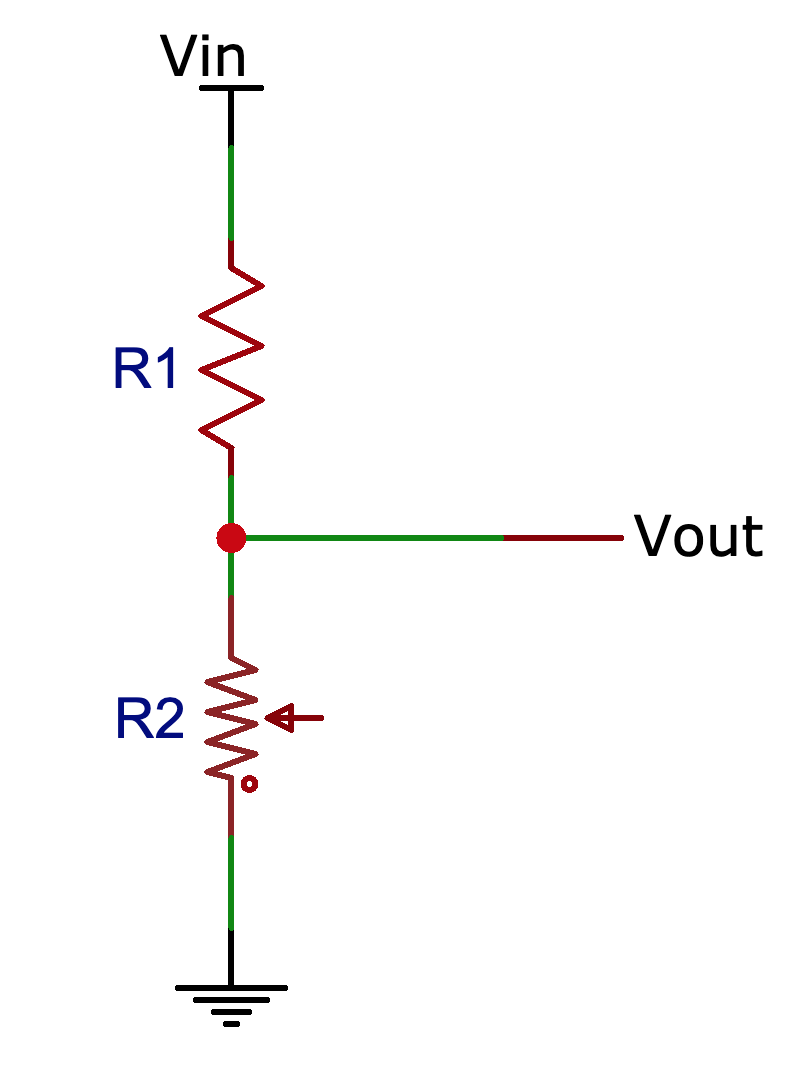
\includegraphics[scale=0.5]{images/lab1_1.png}
    \captionof{figure}{A schematic for a voltage divider}
    \label{fig:first}
    \medskip
\endgroup

\noindent A potentiometer is a variable resistor used to create an adjustable voltage divider. Depending on its position in the circuit, Equation \ref{eq:voltage} can be used to determine the output voltage.   

\begin{equation}
V_{out} = V_{in} (\frac{R\textsubscript{1}}{R\textsubscript{1} + R\textsubscript{2}})
\label{eq:voltage}
\end{equation}


\smallskip
\section{Experimentation}
\subsection{Simple Voltage Divider}

\noindent Using a multimeter, the resistance of the two provided resistors was measured. $R_1$ was measured to be 1K\ohm, while $R_2$ was measured as 5K\ohm. Two cables from the VIN (at 5V) and ground of a DC power supply were connected to the appropriate power rails on the breadboard. $R_1$ and $R_2$ were connected in series, with the positive terminal of the multimeter connected to VIN and the negative terminal connected to in between $R_1$ and $R_2$ (see Figure \ref{fig:second}).

\begingroup
    \medskip
    \centering
    %width=\columnwidth
    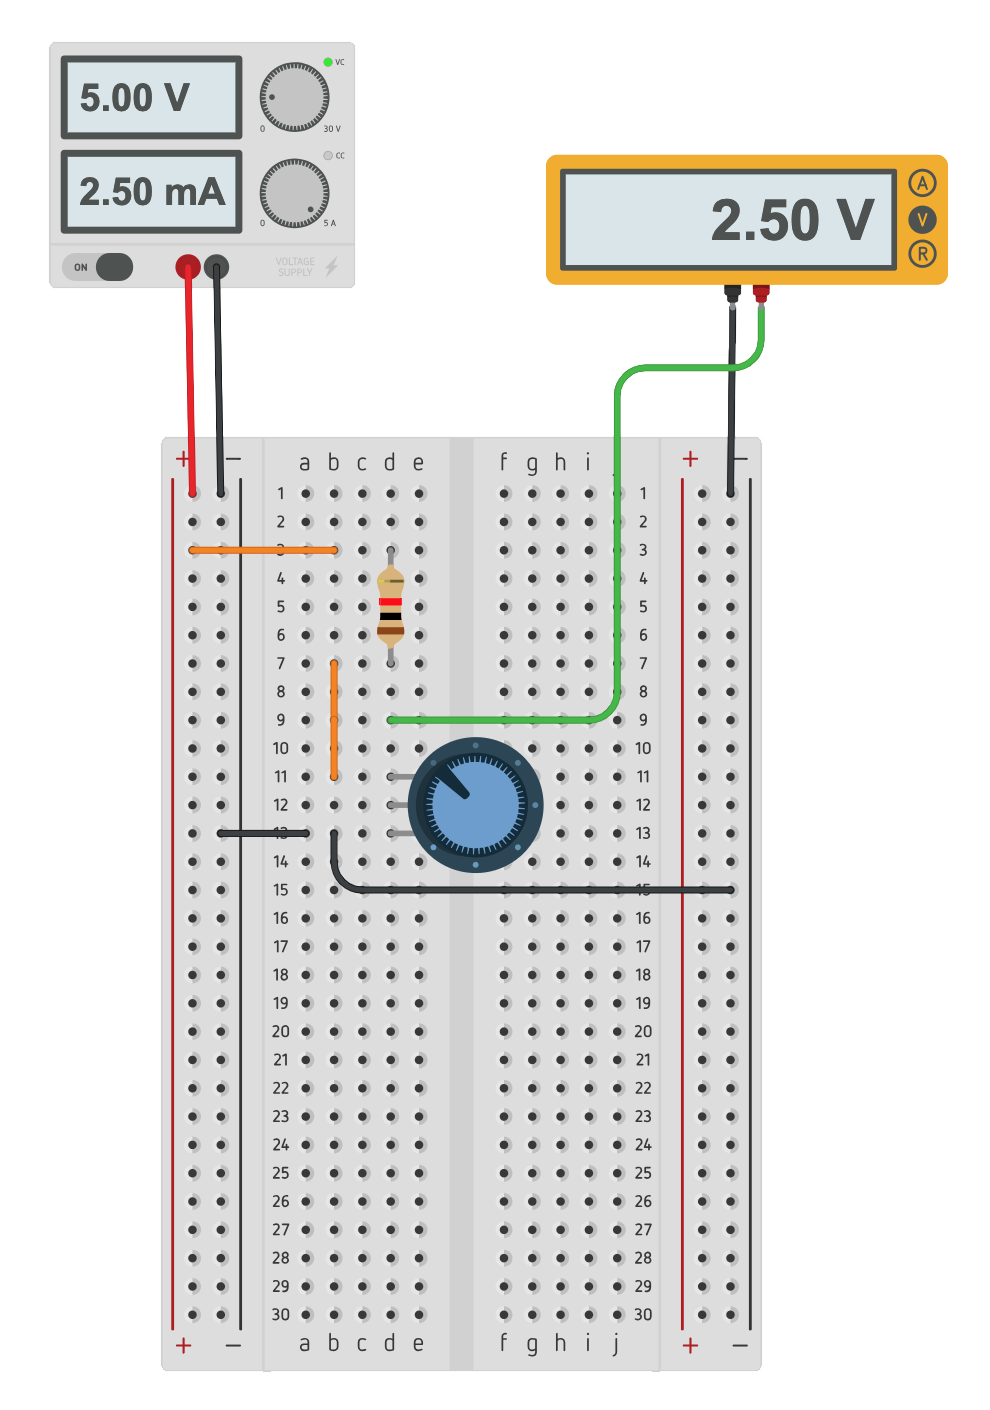
\includegraphics[scale=0.3]{images/lab1_2.png}
    \captionof{figure}{A layout for a simple voltage divider}
    \label{fig:second}
    \medskip
\endgroup

\begingroup
    \medskip
    \centering
    %width=\columnwidth
    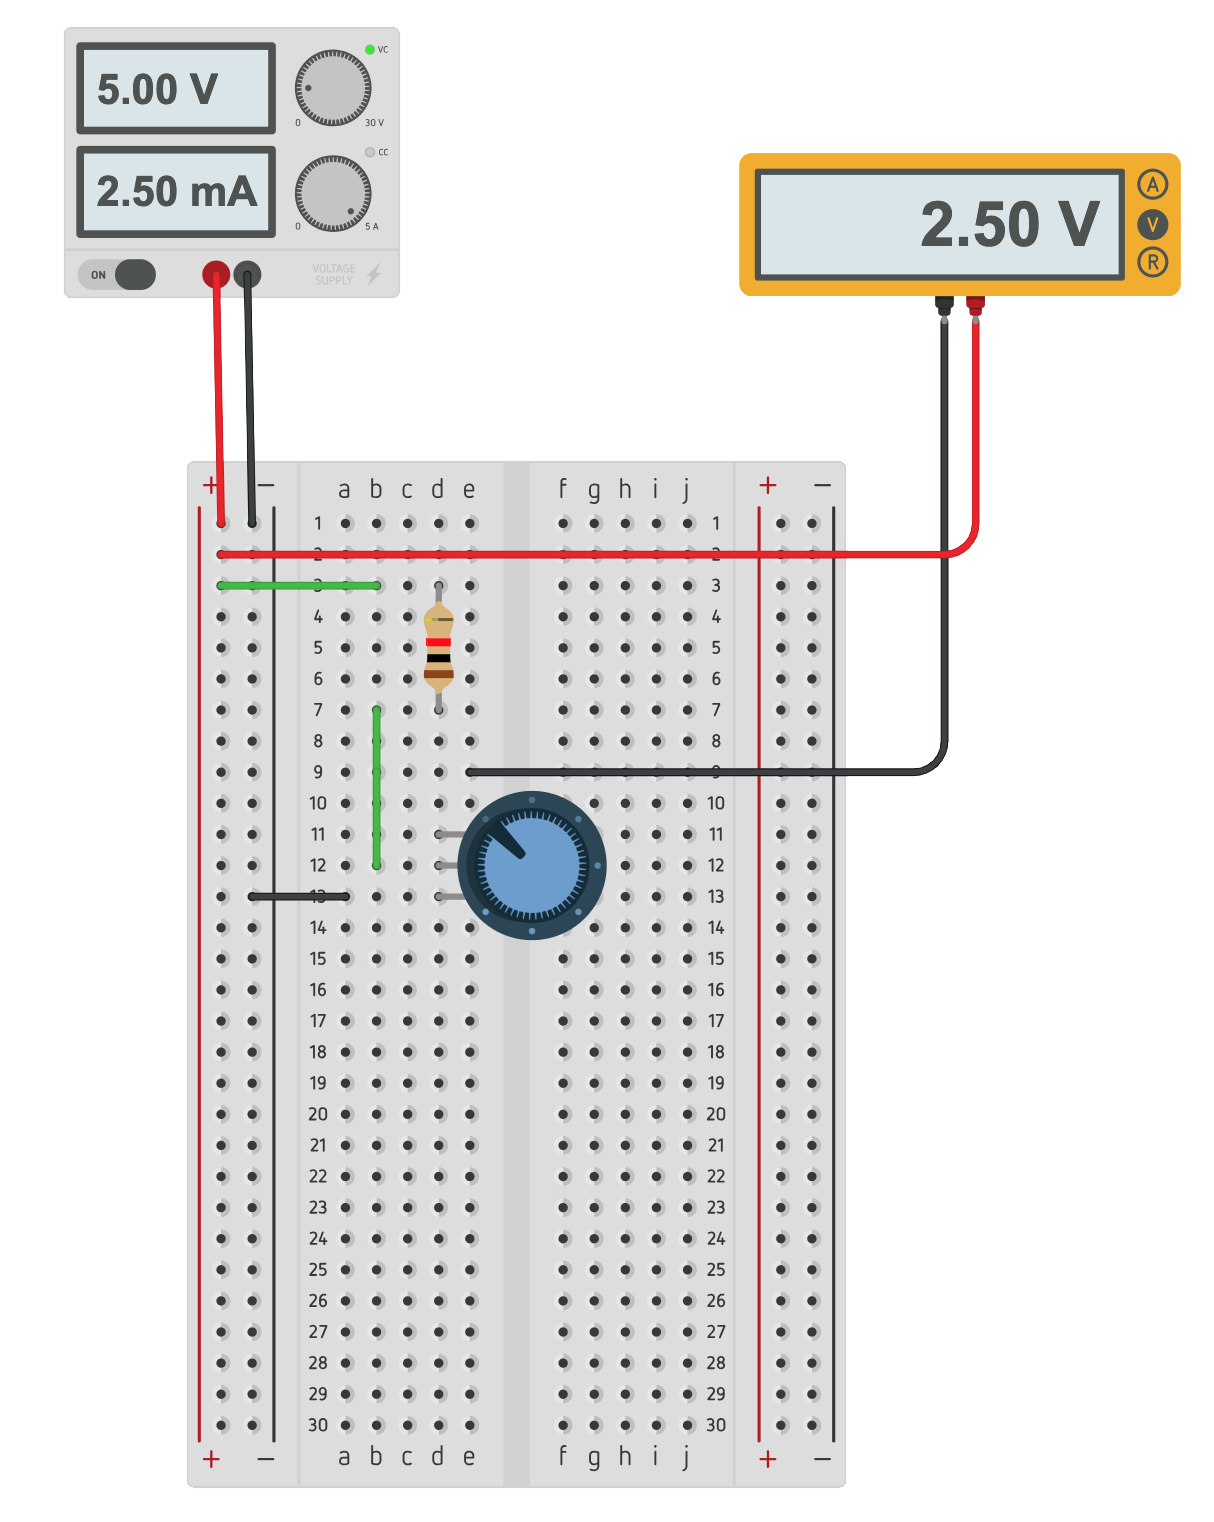
\includegraphics[scale=0.3]{images/lab1_3.png}
    \captionof{figure}{A layout for an adjustable voltage divider}
    \label{fig:third}
    \medskip
\endgroup

\noindent The $V_{out}$ for the simple voltage divider was calculated as follows:

\begin{equation}
V_{out} = V_{in} (\frac{R\textsubscript{1}}{R\textsubscript{1} + R\textsubscript{2}}) = 5V (\frac{1K\ohm}{1K\ohm + 5K\ohm}) = 833 mV
\label{eq:simplevout}
\end{equation}

\medskip


\subsection{Adjustable Voltage Divider}\\

\noindent Similarly constructed, the adjustable voltage divider used a 1K potentiometer for $R_2$ and $R_1$ was measured to be 1K\ohm. The middle pin of the potentiometer was connected to VIN and the third pin connected to common ground. The positive terminal of the multimeter was connected to VIN and the negative terminal was connected to in between $R_1$ and $R_2$ (see Figure \ref{fig:third}).\\ 

\noindent The $V_{out}$ for the adjustable voltage divider (as pictured in Figure \ref{fig:third} was calculated as follows:

\begin{equation}
V_{out} = V_{in} (\frac{R\textsubscript{1}}{R\textsubscript{1} + R\textsubscript{2}}) = 5V (\frac{1K\ohm}{1K\ohm + 1K\ohm}) = 2.5 V
\label{eq:adjustvout}
\end{equation}

\noindent Figure \ref{fig:fourth} shows the breadboard prototype of the adjustable voltage divider. The knob on the potentiometer was tuned to produce a different output voltage.

 \medskip

\begingroup
    \medskip
    \centering
    %width=\columnwidth
    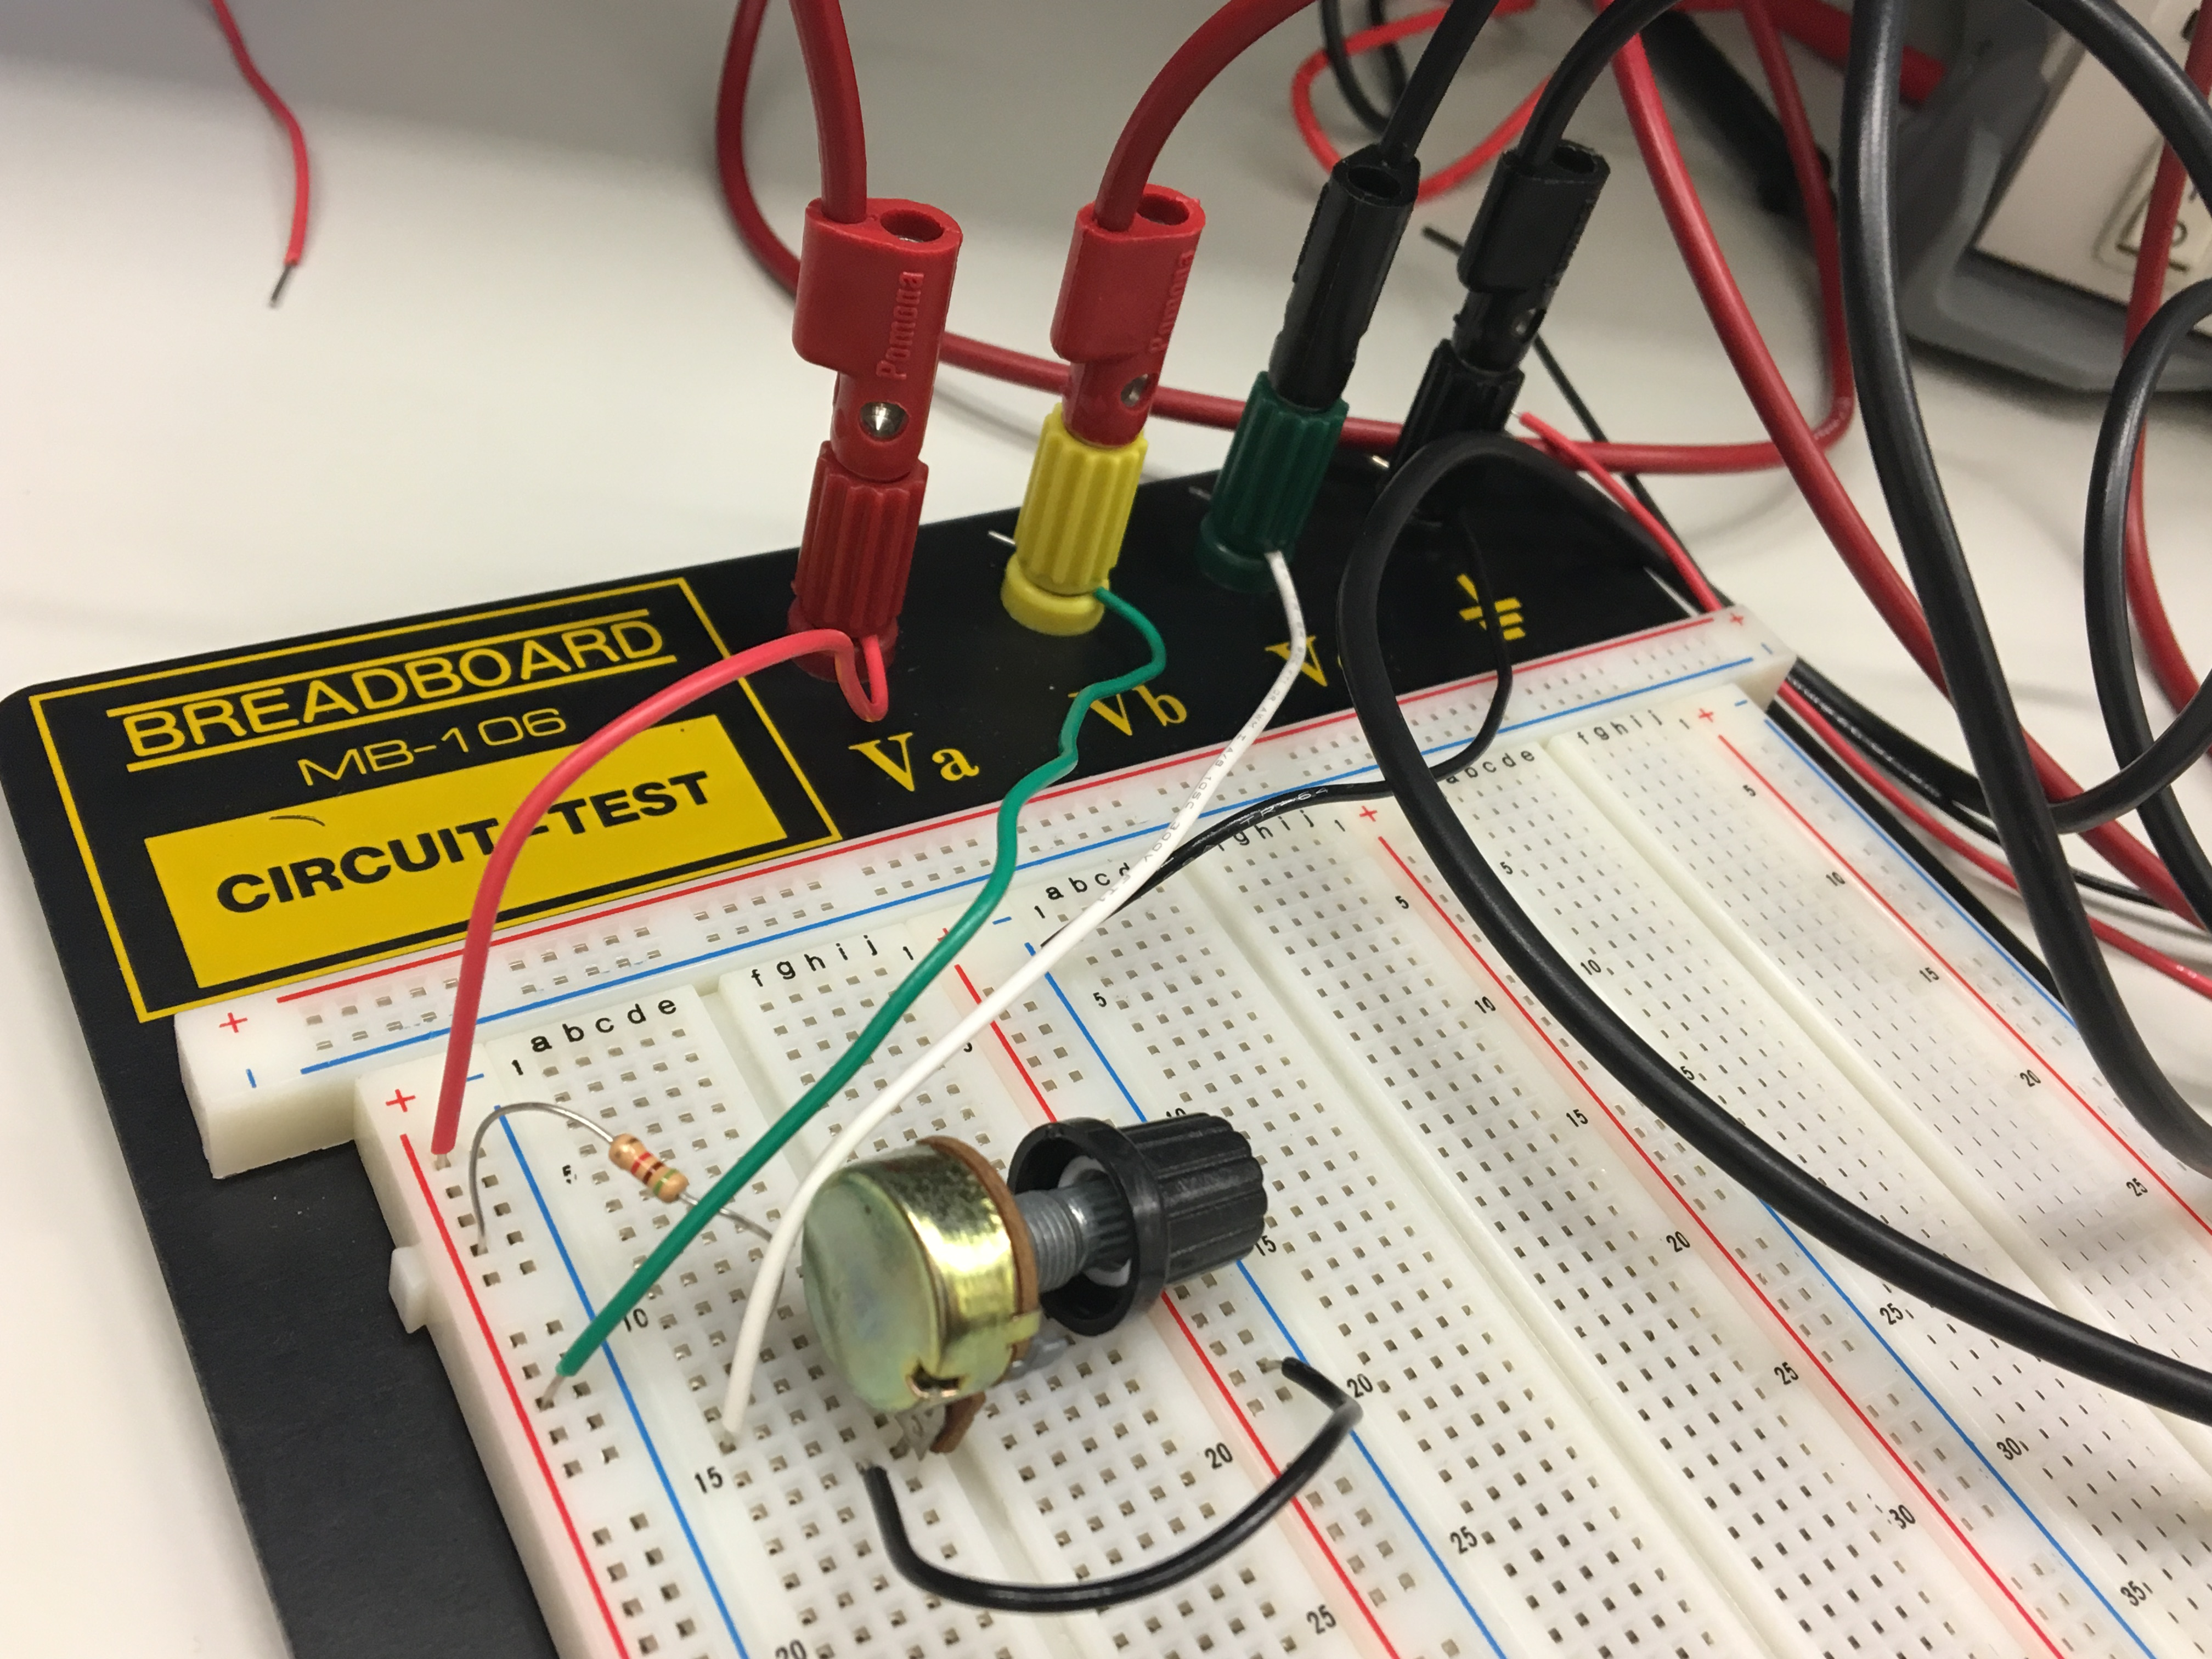
\includegraphics[width =\columnwidth]{images/lab1_4.jpg}
    \captionof{figure}{Breadboard prototype of the adjustable voltage divider}
    \label{fig:fourth}
    \medskip
\endgroup

\section{Discussion and Conclusion}\\

\noindent It was assumed that the $V_{out}$ was to be calculated relative to ground. Thus, in a few of the initial trials, the output voltage reading from the multimeter was $V_{in} - V_{out}$, causing some confusion. It was learned that in order to calculate $V_{out}$ relative to ground, the numerator in Equation \ref{eq:voltage} would have to be $R_2$. However, the task was to calculate relative to VIN, leading the multimeter's terminals to be relocated. 




%\appendices
%\section{Proof of the First Zonklar Equation}
%Appendix one text goes here.

%\section*{Acknowledgment}

\printbibliography



\end{document}